\PassOptionsToPackage{unicode=true}{hyperref} % options for packages loaded elsewhere
\PassOptionsToPackage{hyphens}{url}
\documentclass[11pt,dvipsnames,ignorenonframetext,aspectratio=169]{beamer}
\IfFileExists{pgfpages.sty}{\usepackage{pgfpages}}{}
\setbeamertemplate{caption}[numbered]
\setbeamertemplate{caption label separator}{: }
\setbeamercolor{caption name}{fg=normal text.fg}
\beamertemplatenavigationsymbolsempty
\usepackage{lmodern}
\usepackage{amssymb,amsmath}
\usepackage{ifxetex,ifluatex}
\usepackage{fixltx2e} % provides \textsubscript
\ifnum 0\ifxetex 1\fi\ifluatex 1\fi=0 % if pdftex
  \usepackage[T1]{fontenc}
  \usepackage[utf8]{inputenc}
\else % if luatex or xelatex
  \ifxetex
    \usepackage{mathspec}
  \else
    \usepackage{fontspec}
\fi
\defaultfontfeatures{Ligatures=TeX,Scale=MatchLowercase}







\fi

  \usetheme[]{monash}

  \usecolortheme{monashwhite}


% A default size of 24 is set in beamerthememonash.sty
  \setbeamerfont{title}{series=\bfseries,parent=structure,size=\fontsize{18pt}{32}}

% Title page
\setbeamertemplate{title page}
{\placefig{-0.01}{-0.01}{width=1.01\paperwidth,height=1.01\paperheight}{fusrekhola\_falls\_kaski\_20210814.jpg}
\begin{textblock}{7.5}(1,2.8)\usebeamerfont{title}
{\color{white}\raggedright\par\inserttitle}
\end{textblock}
\begin{textblock}{7.5}(1,7)
{\color{white}\raggedright{\insertauthor}\mbox{}\\[0.2cm]
\insertdate}
\end{textblock}}


  \useinnertheme{rounded}

  \useoutertheme{smoothtree}

% use upquote if available, for straight quotes in verbatim environments
\IfFileExists{upquote.sty}{\usepackage{upquote}}{}
% use microtype if available
\IfFileExists{microtype.sty}{%
  \usepackage{microtype}
  \UseMicrotypeSet[protrusion]{basicmath} % disable protrusion for tt fonts
}{}


\newif\ifbibliography
  \usepackage[round]{natbib}
  \bibliographystyle{plainnat}


\hypersetup{
      pdftitle={Defence mechanisms against pathogens, parasites, insects},
            colorlinks=true,
    linkcolor=red,
    citecolor=Blue,
    urlcolor=lightgrayd,
    breaklinks=true}
%\urlstyle{same}  % Use monospace font for urls







% Prevent slide breaks in the middle of a paragraph:
\widowpenalties 1 10000
\raggedbottom

  \AtBeginPart{
    \let\insertpartnumber\relax
    \let\partname\relax
    \frame{\partpage}
  }
  \AtBeginSection{
    \ifbibliography
    \else
      \let\insertsectionnumber\relax
      \let\sectionname\relax
      \frame{\sectionpage}
    \fi
  }
  \AtBeginSubsection{
    \let\insertsubsectionnumber\relax
    \let\subsectionname\relax
    \frame{\subsectionpage}
  }



\setlength{\parindent}{0pt}
\setlength{\parskip}{6pt plus 2pt minus 1pt}
\setlength{\emergencystretch}{3em}  % prevent overfull lines
\providecommand{\tightlist}{%
  \setlength{\itemsep}{0pt}\setlength{\parskip}{0pt}}

  \setcounter{secnumdepth}{0}


%% Monash overrides
\AtBeginSection[]{
   \frame<beamer>{
   \frametitle{Outline}\vspace*{0.2cm}
   
   \tableofcontents[currentsection,hideallsubsections]
  }}

% Redefine shaded environment if it exists (to ensure text is black)
\ifcsname Shaded\endcsname
  \definecolor{shadecolor}{RGB}{225,225,225}
  \renewenvironment{Shaded}{\color{black}\begin{snugshade}\color{black}}{\end{snugshade}}
\fi
%%


  \usepackage{setspace}
  \usepackage{wasysym}
  % \usepackage{footnote} % don't use this this breaks all
  \usepackage{fontenc}
  \usepackage{fontawesome}
  \usepackage{booktabs,siunitx}
  \usepackage{longtable}
  \usepackage{array}
  \usepackage{multirow}
  \usepackage{wrapfig}
  \usepackage{float}
  \usepackage{colortbl}
  \usepackage{pdflscape}
  \usepackage{tabu}
  \usepackage{threeparttable}
  \usepackage{threeparttablex}
  \usepackage[normalem]{ulem}
  \usepackage{makecell}
  \usepackage{xcolor}
  \usepackage{tikz} % required for image opacity change
  \usepackage[absolute,overlay]{textpos} % for text formatting
  \usepackage{chemfig}
  \usepackage[skip=0.333\baselineskip]{caption}
  % \newcommand*{\AlignChar}[1]{\makebox[1ex][c]{\ensuremath{\scriptstyle#1}}}%
  \usepackage{siunitx}

  % this font option is amenable for beamer
  \setbeamerfont{caption}{size=\tiny}
  \singlespacing
  \definecolor{lightgrayd}{gray}{0.95}
  \definecolor{skyblued}{rgb}{0.65, 0.6, 0.94}
  \definecolor{oranged}{RGB}{245, 145, 200}

  % % better to insert it into template itself
  % \newlength{\cslhangindent}
  % \setlength{\cslhangindent}{1.5em}
  % \newenvironment{cslreferences}%
  %   {\setlength{\parindent}{0pt}%
  %   \everypar{\setlength{\hangindent}{\cslhangindent}}\ignorespaces}%
  %   {\par}

  \usepackage[caption=false]{subfig}

  \newcommand{\bcolumns}{\begin{columns}[T, onlytextwidth]}
  \newcommand{\ecolumns}{\end{columns}}

  \newcommand{\bdescription}{\begin{description}}
  \newcommand{\edescription}{\end{description}}

  \newcommand{\bitemize}{\begin{itemize}}
  \newcommand{\eitemize}{\end{itemize}}
  \AtBeginSubsection{}
  \newcommand{\bsmall}{\begin{small}}
  \newcommand{\esmall}{\end{small}}

  \title[]{Defence mechanisms against pathogens, parasites, insects}


  \author[
        \vspace{-0.5cm}Deependra Dhakal\\
Assistant Professor\\
Agriculture and Forestry University\\
\textit{ddhakal.rookie@gmail.com}\\
\url{https://rookie.rbind.io}
    ]{\vspace{-0.5cm}Deependra Dhakal\\
Assistant Professor\\
Agriculture and Forestry University\\
\textit{ddhakal.rookie@gmail.com}\\
\url{https://rookie.rbind.io}}


\date[
      
  ]{
    }

\begin{document}

% Hide progress bar and footline on titlepage
  \begin{frame}[plain]
  \titlepage
  \end{frame}


   \frame<beamer>{
   \frametitle{Outline}\vspace*{0.2cm}
   
   \tableofcontents[hideallsubsections]
  }

\hypertarget{defense-mechanism-against-pathogens-and-parasites}{%
\section{Defense mechanism against pathogens and
parasites}\label{defense-mechanism-against-pathogens-and-parasites}}

\begin{frame}{Disease escape or avoidance}
\protect\hypertarget{disease-escape-or-avoidance}{}
\begin{itemize}
\tightlist
\item
  Not even a true resistance mechanism

  \begin{itemize}
  \tightlist
  \item
    maturing plants may complete their growth and produce seeds before
    epidemics of foliar diseases have progressed far enough to cause
    significant damage
  \end{itemize}
\item
  Wheat stem rust epidemics in US begin with overwintered infections in
  winter wheat plants near the Gulf Coast. \textit{P. graminis} develops
  best in warm weather, so stem rust epidemics develop slowly during the
  spring. One reason for the decline of stem rust damage in the Central
  Plains states of Oklahoma and Kansas was the switch to earlier
  maturing winter wheat cultivars in those states in the 1930s and
  1940s.
\item
  Reduction in the population density of host plants
\end{itemize}
\end{frame}

\begin{frame}{}
\protect\hypertarget{section}{}
\begin{itemize}
\tightlist
\item
  Morphological feature of plants enabling them to avoid infection
\item
  Tuber rot in stored potatoes is initiated primarily in wounds to the
  tubers incurred during harvesting/transport. Rapid healing by
  development of a suberized layer over the wounded tissue is considered
  most critical aspect of resistance therein.
\item
  Floral development is important in the resistance of wheat to ergot
  caused by \textit{Claviceps purpurea}.

  \begin{itemize}
  \tightlist
  \item
    pathogen invades the ovules by way of stigmas of the rye florets
  \item
    \(\because\) rye is typically cross-pollinated, the unfertilized
    stigmas are exposed to ascospores
  \item
    however, once ovules are fertilized, stigmas are no longer receptive
    to infection
  \item
    \(\because\) wheat is self-pollinated, stigmas are no longer
    receptive to infection by the time they become exposed to pathogen
    spores in air
  \item
    male sterile lines of wheat tend to be infected heavily as rye by
    ergot!
  \end{itemize}
\end{itemize}
\end{frame}

\begin{frame}{}
\protect\hypertarget{section-1}{}
\begin{itemize}
\tightlist
\item
  Failure of anther extrusion in barley cultivars leads to partial
  escape from Fusarium head blight.
\item
  Covering of leaf epidermis with hairs or waxes that repel water
\item
  Upright geometry of foliage cause water droplets to roll off the
  leaves allowing them to dry rapidly
\item
  Plants unattractive to potential vectors escape infection even if they
  are susceptible to the vector-borne pathogen
\item
  Rice cultivars selected for more efficient silicon uptake have
  morphological resistance to \textit{M. grisea} (mentioned earlier).
\item
  In wheat stem rust caused by \textit{P. graminis}:

  \begin{itemize}
  \tightlist
  \item
    seedlings exhibit no morphological resistance
  \item
    adult plants allow growth of pathogen only in the chlorophyllous
    collenchyma bundles of stems
  \item
    cultivars with narrow, isolated strands of collenchyma bundles
    separated by broad bands of sclerenchyma are partially resistant to
    stem rust in adult plants
  \end{itemize}
\end{itemize}
\end{frame}

\begin{frame}{Resistance}
\protect\hypertarget{resistance}{}
\begin{itemize}
\tightlist
\item
  Ability of plant to reduce the growth and/or development of the
  parasite after contact has been initiated or established.
\item
  Mechanisms of resistance are better suited against pathogen and
  endoparasites, rather than herbivores.
\item
  In ecological terms, resistance is occurs in the events of
  antibiosis\footnote[frame]{A biological interaction between two organisms that is deterimental to at least one of them.}
\item
  Various pathogens are susceptible to a broad range of chemical defense
  compounds (owing to their antibiotic properties):

  \begin{itemize}
  \tightlist
  \item
    tannins
  \item
    phenolic compounds
  \item
    dienes
  \item
    saponins
  \item
    proteases
  \item
    hydrolytic enzymes
  \end{itemize}
\item
  Seeds typically have higer concentration of antibiotic compounds than
  vegetaive parts of annual plants
\end{itemize}
\end{frame}

\begin{frame}{Tolerance}
\protect\hypertarget{tolerance}{}
\begin{itemize}
\tightlist
\item
  A mechanism that enables plants to recover from infection or herbivory
  inflicted damage thus leading to milder form of symptoms.
\item
  In virology, when the virus concentration in the plants is relatively
  high, the conclusion that the plants are tolerant is justified.
\end{itemize}
\end{frame}

\begin{frame}{Induced response to invasion}
\protect\hypertarget{induced-response-to-invasion}{}
\footnotesize

\begin{itemize}
\tightlist
\item
  Plants respond to woulds in a non-specific production of corky tissue
  that wall off the broken area of the epidermis. Similar barriers are
  produced in the woody stems and roots of trees or other perennial
  plants in response to canker-forming pathogens.

  \begin{itemize}
  \tightlist
  \item
    speed at which a plant produces such barrier is a measure of its
    generalized resistance
  \end{itemize}
\item
  Cell walls in the epidermis may induce thickenings in reponse to
  pathogens attempting to penetrate their outer walls.

  \begin{itemize}
  \tightlist
  \item
    walls thickenings are often infused with phenolic substances
  \end{itemize}
\item
  Wilt disease fungi typically grow through the xylem and tend to cut
  off water flow to aerial parts of the plant

  \begin{itemize}
  \tightlist
  \item
    plant may wall off the pathogen by forming tyloses within xylem
    cells
  \end{itemize}
\item
  Plants activate pathways to produce characteristic antibiotic
  compounds called phytoalexins in the cells around the site of attack

  \begin{itemize}
  \tightlist
  \item
    if the response is soon enough and extensive, plant may display
    partial resistance
  \end{itemize}
\item
  The rate of response of the host may depend on its ability to
  recognize that it is being invaded.
\end{itemize}
\end{frame}

\begin{frame}{}
\protect\hypertarget{section-2}{}
\begin{description}
\item[Systemic acquired resistance] An induced defense in host may confer long lasting protection against a broad spectrum of micro-organisms (i.e. viral, bacterial, and fungal)
\end{description}

\begin{itemize}
\tightlist
\item
  Enhanced resistance against subsequent attack by a wide array of
  pathogen.
\item
  As in partial/horizontal resistance, SAR takes 24-48 hours to onset
  and can last for several months.
\item
  It may be induced by certain synthetic chemicals, \emph{viz}.
  salicylic acid, 2,6-dichloroisonicotinic acid (INA) and benzo (1,2,3)
  thiadiazole-7-carbothioic acid-S-methyl ester (BTH).
\item
  Pathogen recognition triggers a number of rapid cellular responses,
  including ionic changes and phosphorylation cascades, which preced the
  accumulation of reactive oxygen species (ROS), nitric acid (NO) and
  salicylic acid (SA) and transcriptional activation of defense related
  gene.
\item
  Through epigenetic changes in the host genome, the resistance may be
  transmitted across generations.
\end{itemize}
\end{frame}

\begin{frame}{}
\protect\hypertarget{section-3}{}
\begin{itemize}
\tightlist
\item
  In many cases of host-pathogen interaction, genes in one organism are
  triggered to be expressed by a substance produced by the other
  organism. For example,

  \begin{itemize}
  \tightlist
  \item
    genes for cell wall-degrading enzymes in the pathogen are induced by
    the presence of monomers or oligomers of host cell wall
    macromolecules that are substrates for these enzymes.
  \item
    genes for defense reactions in the host, eg. phytoalexins, are
    triggered to expression by certain signal compounds activated by
    inducer molecules (elicitors) produced by the pathogen.
  \end{itemize}
\end{itemize}
\end{frame}

\hypertarget{genetics-of-disease-and-resistance-mechanism}{%
\section{Genetics of disease and resistance
mechanism}\label{genetics-of-disease-and-resistance-mechanism}}

\begin{frame}{At population and genotypic level}
\protect\hypertarget{at-population-and-genotypic-level}{}
\bcolumns
\column{0.55\textwidth}
\footnotesize

\begin{itemize}
\tightlist
\item
  In order to understand disease, genetics of causal agent need to be
  elucidated
\item
  Characters in individuals including pathogens are variable mostly as a
  result of

  \begin{itemize}
  \scriptsize
  \item Sexual process -- oospores, ascospores and basidiospores (in oomycetes and fungi); seeds of higher plants and eggs of nematodes
  \item Asexual process -- (owing to astronomical number of microorganism individuals produced) conidia, zoospores, sclerotia and uredospores (in fungi); bacteria, mollicutes and viruses
  \end{itemize}
\item
  Sexually reproducing organisms generate variability through
  segregation and recombination of genes, and even in asexually
  reproducing pathogens (bacteria) variants are produced by mutations.
\end{itemize}

\column{0.45\textwidth}

\footnotesize

\begin{itemize}
\tightlist
\item
  Factors affecting gene flow and genotype fitness are major drivers for
  evolution of both plant pathogen and host
  population\footnote[frame]{\scriptsize Refer to lecture notes of Population Genetics on factor affecting gene and genotype frequency changes}.
\item
  Reproductive cycle of pathogen vary considerably, with oomycetes and
  fungi having some of the most complex reproduction systems.
\end{itemize}

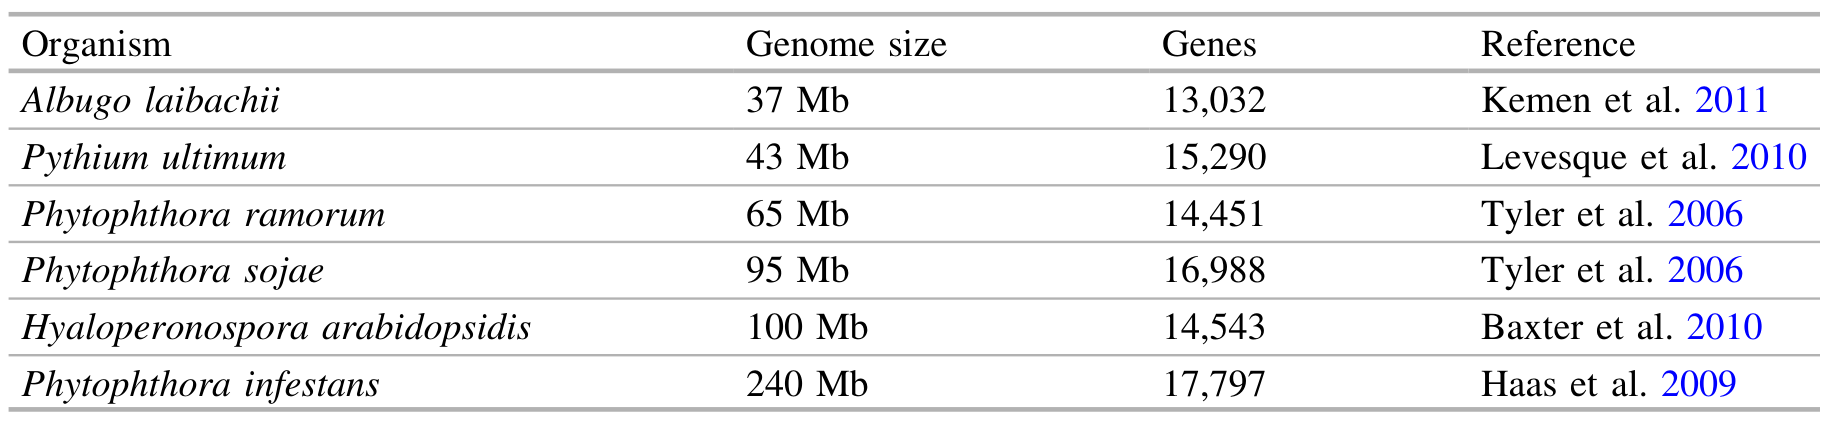
\includegraphics[width=0.88\linewidth]{../images/genome-complexity-comparison-oomycete}

\ecolumns
\end{frame}

\begin{frame}{At genetic level}
\protect\hypertarget{at-genetic-level}{}
\footnotesize

\begin{itemize}
\tightlist
\item
  Genetic information (determines the form and function) is encoded as
  DNA or (exceptionally) RNA.

  \begin{itemize}
  \scriptsize
  \item Nucleus (follows Mendalian inheritance)
  \item Mitochondria -- susceptibility genes for southern corn leaf blight caused by \textit{Bipolaris maydis} and yellow leaf blight caused by \textit{Phyllosticta maydis}
  \item Plasmid (autonomously replicating)
  \item Chloroplasts
  \end{itemize}
\item
  A gene (in general) is characterized by:

  \begin{itemize}
  \scriptsize
  \item 100-500 codon triplets
  \item Coding and and non-coding region
  \item Protein or RNA as code product
  \end{itemize}
\item
  Genetic processes

  \begin{itemize}
  \scriptsize
  \item Replication
  \item Transcription
  \item Translation
  \item Regulatory elements -- promoters, enhancers, silencers or terminators
  \end{itemize}
\end{itemize}
\end{frame}

\begin{frame}{Genetic fine structure of resistance loci}
\protect\hypertarget{genetic-fine-structure-of-resistance-loci}{}
Refer to Chapter 2 of \citet{hulbert1997genetic}.
\end{frame}

\begin{frame}{Mechanism of infection by bacteria and fungi}
\protect\hypertarget{mechanism-of-infection-by-bacteria-and-fungi}{}
\begin{figure}

{\centering 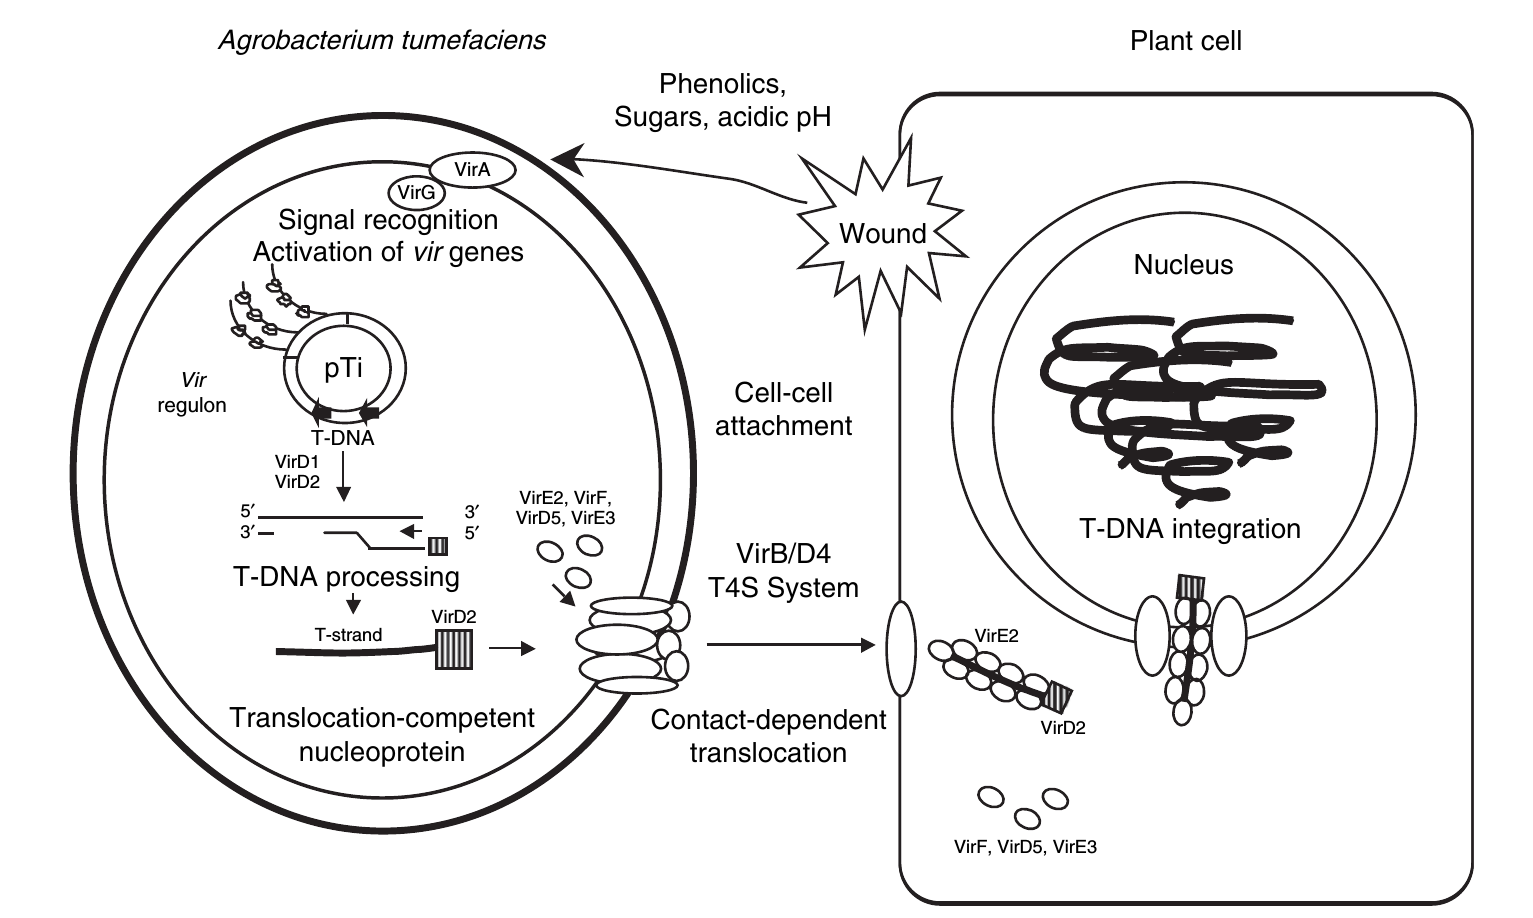
\includegraphics[width=0.66\linewidth]{../images/agrobacterium-transformation} 

}

\caption{Overview of agrobacterium tumefaciens infection process. Upon activation of the VirA/VirG two-component signal transduction system by signals released from wounded plant cells, a single-strand transferred DNA (T-DNA) is processed from the Ti plasmid and delivered as a nucleoprotein complex (T-complex) to plant nuclei. Expression of T-DNA genes in the plant result in the loss of cell growth control and tumor formation.}\label{fig:mechanism-of-infection}
\end{figure}
\end{frame}

\begin{frame}{Defense mechanisms against bacteria and fugi}
\protect\hypertarget{defense-mechanisms-against-bacteria-and-fugi}{}
\begin{itemize}
\tightlist
\item
  Mitochondrial genes of some corn varieties (Texas male-sterile
  cytoplasm) renders plant susceptible to Bipolaris as the host plant
  encodes for a receptor that binds to the corresponding toxin produced
  by the pathogen.
\end{itemize}
\end{frame}

\begin{frame}{Mechanism of virus infection}
\protect\hypertarget{mechanism-of-virus-infection}{}
\end{frame}

\begin{frame}{Defense mechanisms against virus}
\protect\hypertarget{defense-mechanisms-against-virus}{}
\begin{itemize}
\tightlist
\item
  Refer to Chapter 6, Plant-virus interactions: Defense and
  counter-defense \citet{lewsey2009plant} (Annual Plant Reviews, Volume
  34).
\end{itemize}
\end{frame}

\begin{frame}{}
\protect\hypertarget{section-4}{}
\begin{center}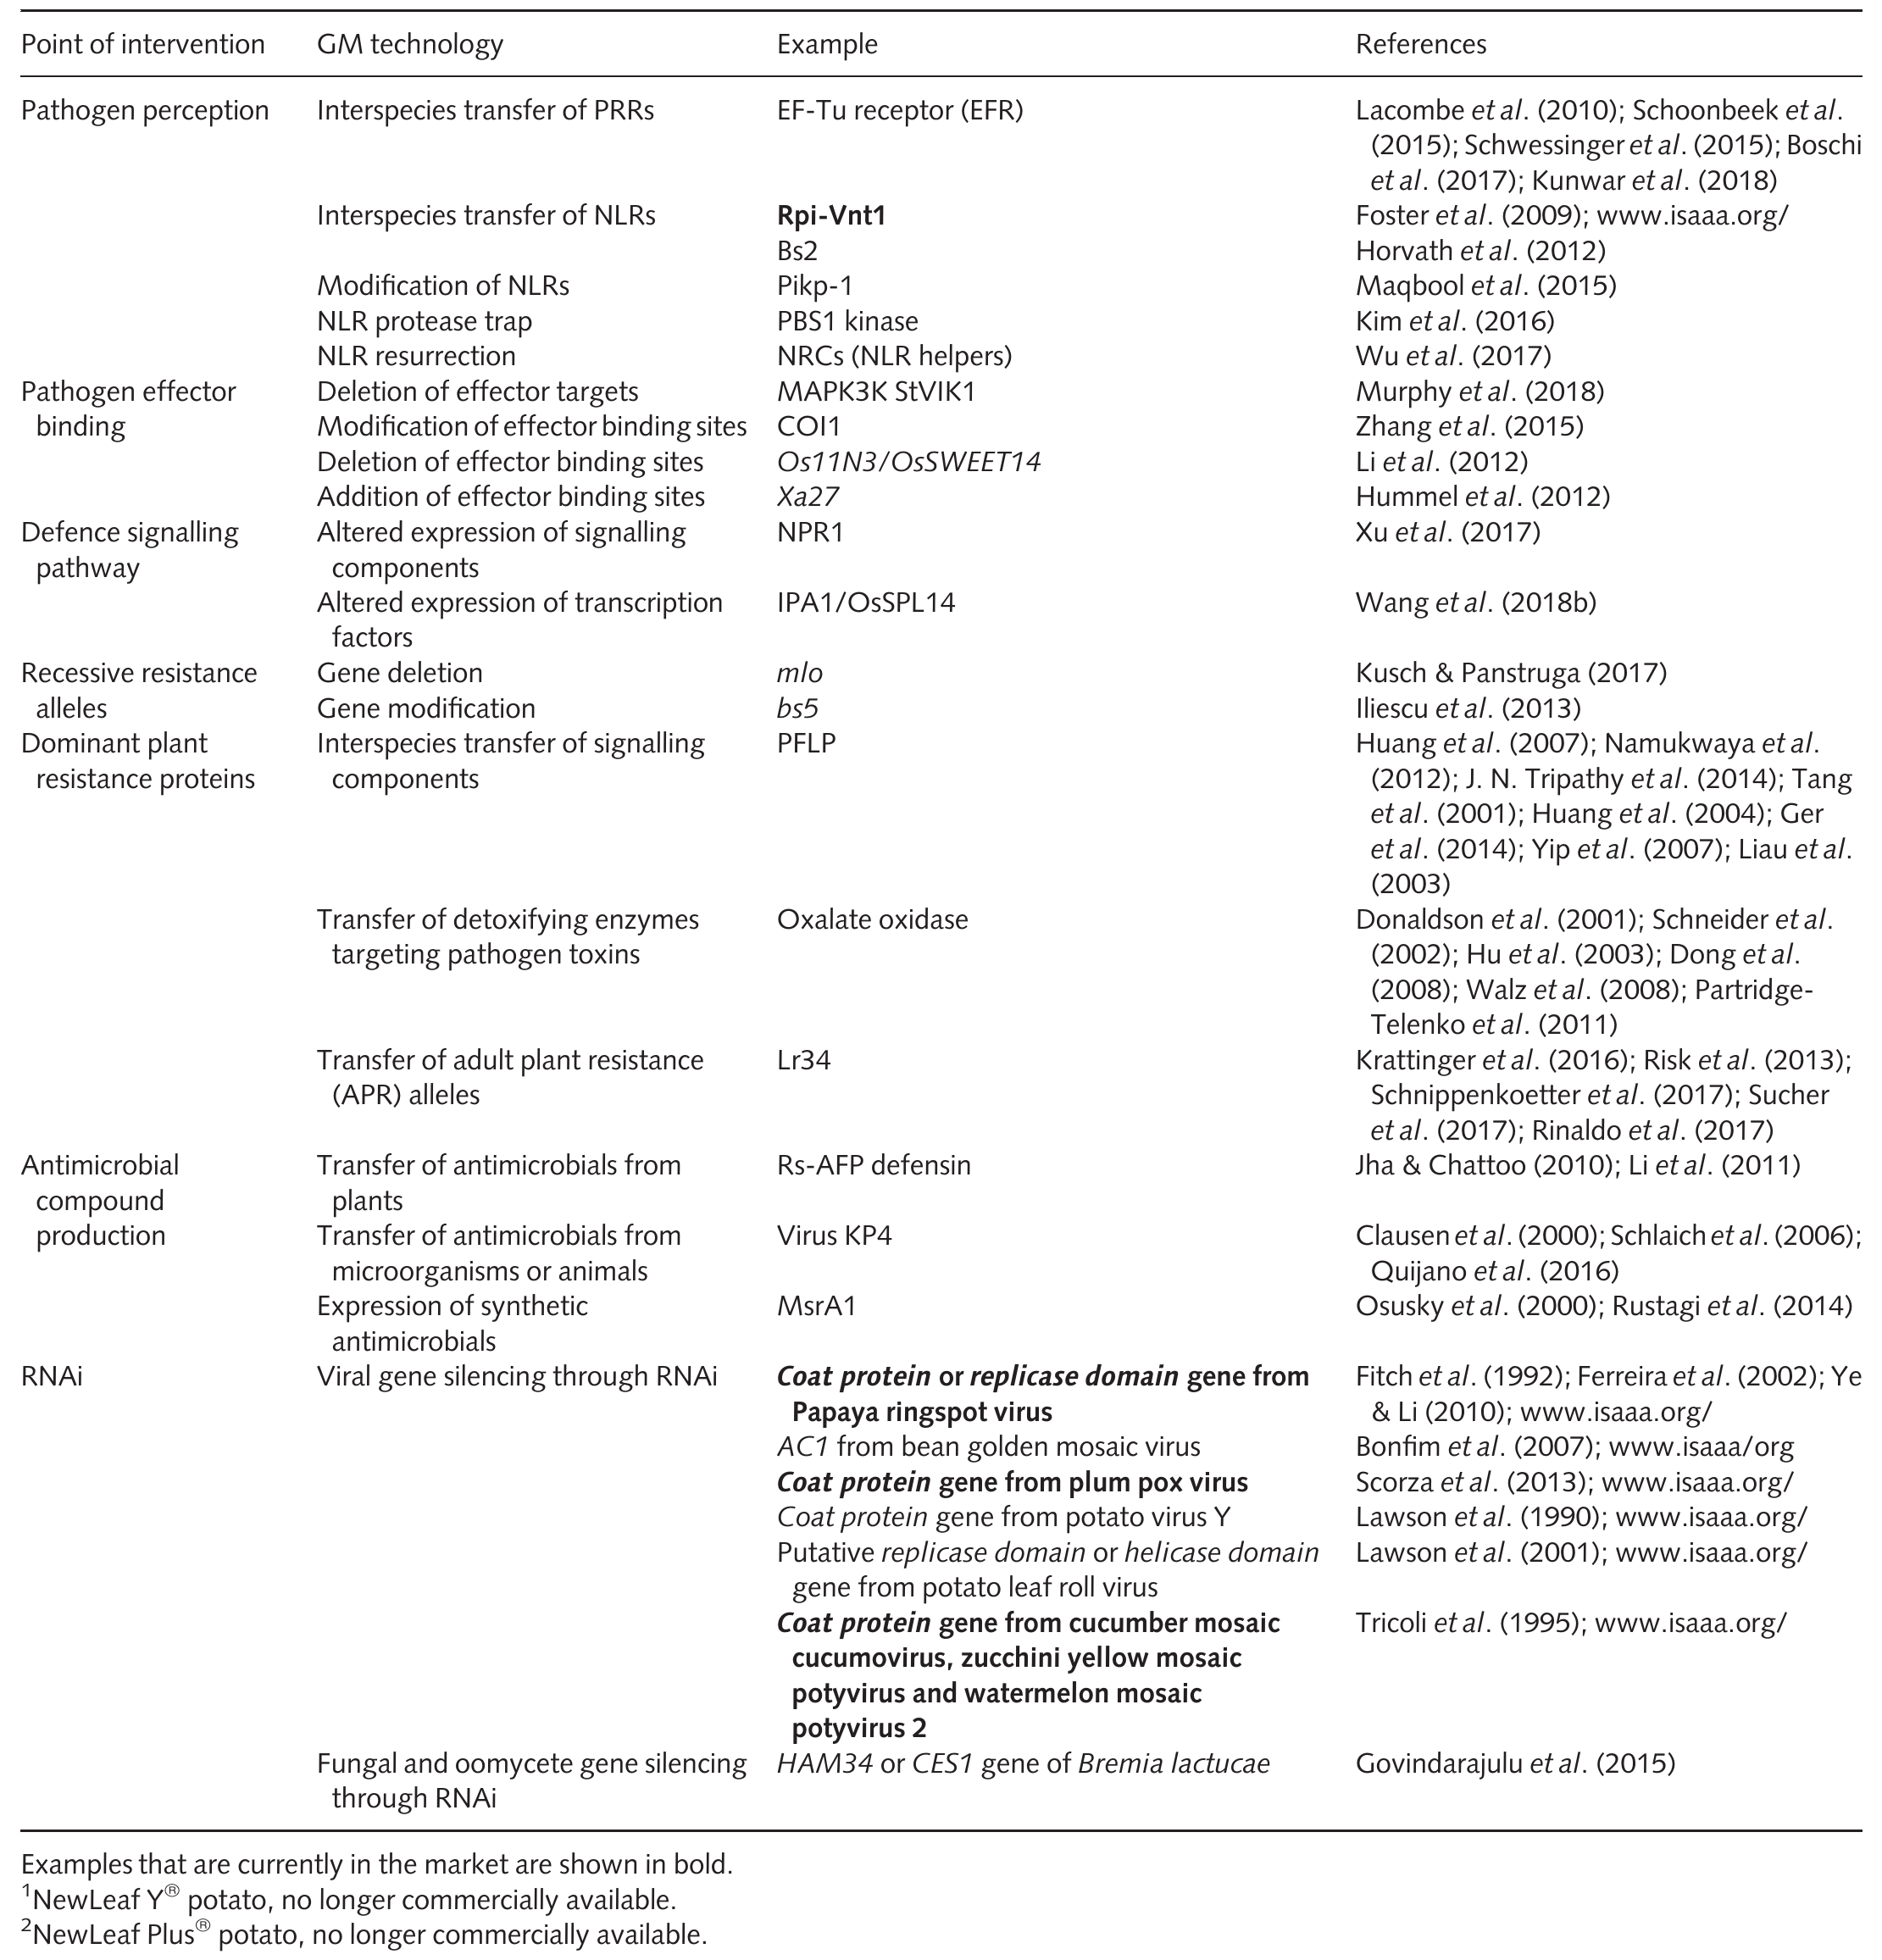
\includegraphics[width=0.4\linewidth]{../images/genetic_solution_pathogens} \end{center}

\tiny (Note: Refer to \citep{van2020genetic} for more on topic: Genetic
modification to improve disease resistance in crops.
\end{frame}

\hypertarget{defense-mechanisms-against-insects-and-herbivory}{%
\section{Defense mechanisms against insects and
herbivory}\label{defense-mechanisms-against-insects-and-herbivory}}

\begin{frame}{Non preference/non-acceptance/antixenosis}
\protect\hypertarget{non-preferencenon-acceptanceantixenosis}{}
\footnotesize

\begin{itemize}
\tightlist
\item
  Term `antixenosis' was first used to refer to non-preference by Kogan
  and Ortman, 1972.
\item
  Host varieties are unattractive or unsuitable for colonization,
  oviposition or both by an insect pest.
\item
  Insects will not accept resistant host even if there is no alternative
  source of food.
\item
  Non-preference of a host strain is detectable only when the preferred
  host strain is present.
\item
  Degrees of non-preference by insects varies. For example, in aphids,

  \begin{itemize}
  \item insects avoid resistant plants $\longrightarrow$ raspberry
  \item insects feed transiently before appearing restless and walking-off to susceptible hosts $\longrightarrow$ sugarbeet
  \item the striped stem borer moth has a strong preference for oviposition on certain rice varieties. Susceptible varieties receive 10-15 times more egg masses than resistant ones.
  \end{itemize}
\end{itemize}
\end{frame}

\begin{frame}{}
\protect\hypertarget{section-5}{}
\footnotesize

\begin{itemize}
\tightlist
\item
  Non-preference is manifested with respect to activities such as
  colonization, egg laying, feeding, pupation, etc.
\item
  Morphological features of host plant prevent insects from approaching,
  landing, settling, feeding or oviposition.
\item
  Biochemicals (allomones/kairomones) produced by certain plants make
  them more preferable than others

  \begin{itemize}
  \item lower levels of cucurbitacins in fruits fend-off beetles in cucurbits
  \item in rice, brown plant-hoppers attack susceptible rice varieties because of presence of asparagine in relatively higher concentrations 
  \end{itemize}
\item
  Physical factors (shape, size, color, pubescence, tissue
  characteristics and secretions) also cause non-preference
\item
  In polyphagous insect (e.g.~Heliothis zea) non-preference may not be
  an effective mechanism of resistance since the insect will multiply on
  alternate hosts.
\end{itemize}

\scriptsize (Refer to Chapter 9 on Chemical ecology of plant-insect
interaction, \citet{mithofer2009chemical} (Annual Plant Reviews, Volume
34))
\end{frame}

\begin{frame}{Antibiosis}
\protect\hypertarget{antibiosis}{}
\begin{itemize}
\tightlist
\item
  Refers to an adverse effect of feeding on a resistant host plant on
  the development and/or reproduction at various stages (broadly termed
  \emph{life history} factors) of the insect pests
\item
  Effect of continued feeding despite antibiosis range from death of
  instar/nymph or larve, reduction in survival ability of over-wintering
  insects and death of adult insect on the extreme.
\item
  In maize, 2,4-dihydroxy-7-methoxy-1,4-benzoxazine-3-one (DIMBOA) has
  been identified as the biochemical that inhibits the growth of the
  larve of Europen corn borer.
\item
  Type and availability of primary metabolites may also be basis of
  antibiosis as it may cause nutritional imbalance in insect pests,
  e.g.~pea varieties with \(\small\Downarrow\) level of amino acids and
  \(\small\Uparrow\) level of sugar show resistance to pea aphids (
  \emph{Acyrthosiphon pisum})
\end{itemize}
\end{frame}

\begin{frame}{Tolerance}
\protect\hypertarget{tolerance-1}{}
\begin{itemize}
\tightlist
\item
  Insect pest attack the tolerant variety to the same degree as a
  susceptible one, but at the same level of infestation, a tolerant
  variety can compensate for/recover from the damage without loosing the
  yield that the susceptible variety does.
\item
  Involves factors like -- vigor, compensatory growth rate, stage of
  life cycle of crop, wound healing, mechanical support in
  tissues/organs, segment of the crop which incurred damage and
  photosynthate partitioning.
\item
  Tolerant variety of maize (for example) repair and replaces the roots
  damaged by western corn root-worm ( \emph{Diabrotica virgifera}).
\end{itemize}
\end{frame}

\begin{frame}{Genetic basis of resistance to insects}
\protect\hypertarget{genetic-basis-of-resistance-to-insects}{}
\end{frame}

\hypertarget{bibliography}{%
\section{Bibliography}\label{bibliography}}

\begin{frame}{References}
\protect\hypertarget{references}{}
\end{frame}

          \begin{frame}[allowframebreaks]{}
    \bibliographytrue
    \bibliography{./../bibliographies.bib}
    \end{frame}
  


\end{document}
